\documentclass[10pt,letterpaper]{article}
\usepackage[T1]{fontenc}
\usepackage[scaled=0.92]{helvet}
\renewcommand{\ttdefault}{lmtt}
\renewcommand{\familydefault}{\sfdefault}
\usepackage[margin=1in]{geometry}
\usepackage{graphicx,xcolor,booktabs,float,listings,array,amsmath}
\usepackage[hidelinks]{hyperref}
\hypersetup{pdftitle={Bridge Column SDOF Example: Results}}
\setlength{\parindent}{0pt}
\setlength{\parskip}{6pt}
\definecolor{head}{RGB}{15,71,97}
\definecolor{cbg}{RGB}{43,43,43}
\definecolor{cfg}{RGB}{169,183,198}
\definecolor{cstr}{RGB}{106,135,89}
\definecolor{ckw}{RGB}{204,120,50}
\definecolor{ccm}{RGB}{128,128,128}
\makeatletter
\renewcommand\section{\@startsection{section}{1}{\z@}{-2.5ex}{1.2ex}{\Large\bfseries\color{head}}}
\renewcommand\subsection{\@startsection{subsection}{2}{\z@}{-2ex}{0.8ex}{\large\color{head}}}
\makeatother
\lstset{language=Python, basicstyle=\ttfamily\footnotesize\color{cfg}, 
  keywordstyle=\color{ckw}, stringstyle=\color{cstr}, commentstyle=\color{ccm},
  showstringspaces=false, breaklines=true, columns=fullflexible, keepspaces=true,
  aboveskip=0pt, belowskip=0pt}
\newcommand{\codefile}[1]{\par\vspace{2pt}\noindent\colorbox{cbg}{\parbox{\dimexpr\textwidth-2\fboxsep}{\lstinputlisting{#1}}}\par\vspace{2pt}}
\newcommand{\code}[1]{\texttt{#1}}
\newcommand{\figpair}[2]{\begin{figure}[H]\centering
  \fbox{\includegraphics[width=0.47\textwidth]{#1}}\hfill\fbox{\includegraphics[width=0.47\textwidth]{#2}}\end{figure}}
\newcommand{\figone}[2]{\begin{figure}[H]\centering\fbox{\includegraphics[width=#1\textwidth]{#2}}\end{figure}}
\setlength{\fboxsep}{4pt}
\setlength{\fboxrule}{0.3pt}

\begin{document}

{\raggedleft
{\Huge\bfseries Bridge\_Column\_SDOF Example\par}
\vspace{4pt}
{\Large Results from PrelimAnalysis to PSDamHA\par}
\vspace{4pt}
{\small PyPBEE, single-component intensity measure (changes after v1.2.0, not released)\par}
{\small 12 November 2026\par}
}
\vspace{6pt}
{\color{head}\hrule}

\section{Introduction}

This document shows the results of the \code{Bridge\_Column\_SDOF} example in
\code{scripts/examples}. The example is a single-degree-of-freedom (SDOF) version of the
\code{Bridge\_Column} example in the PyPBEE User Manual. The format follows Section 6 of the manual:
each block of code is followed by the figure that it makes.

The example runs the full workflow for analysis case \code{'100'} (deterministic FE model, expected
values of the model parameters):

\begin{center}
PrelimAnalysis $\rightarrow$ PSHA $\rightarrow$ GMS $\rightarrow$ NLTHA $\rightarrow$ PSDemHA $\rightarrow$ PSDamHA
\end{center}

The example is different from \code{Bridge\_Column} in three areas:
\begin{itemize}\setlength{\itemsep}{1pt}
\item The model is one mass and one bilinear spring. The excitation is in one direction.
\item The intensity measure (IM) uses one horizontal component of each record.
\item The EDP is a new class, \code{MaxDisp}, in the example folder. The DS uses this EDP.
\end{itemize}

\section{SDOF Model}

The properties of the SDOF come from the as-designed \code{Bridge\_Column} model (column diameter
5.51 ft, longitudinal steel ratio 0.02, expected material properties). A static pushover of that
model gives the yield force.

\begin{center}
\begin{tabular}{llll}
\toprule
Parameter & Name in the model & Value & Source \\
\midrule
Weight & \code{W} & 3143 kip & Deck weight plus half of the column weight \\
Stiffness & \code{k\_in\_kip\_per\_in} & 363 kip/in & Gives the $T_1$ of \code{Bridge\_Column} \\
Yield force & \code{Fy\_in\_kip} & 465 kip & Peak base shear of the pushover \\
Hardening ratio & \code{b} & 0.01 & Same as \code{Bridge\_Column} \\
Damping ratio & \code{damp\_ratio} & 0.01 & Same as \code{Bridge\_Column} \\
\bottomrule
\end{tabular}
\end{center}

\code{k} and \code{Fy} are the primary design parameters, with one design point. \code{W}, \code{b}
and \code{damp\_ratio} are the random model parameters. PrelimAnalysis gives $T_1$ = 0.9405 s. The
$T_1$ of \code{Bridge\_Column} is 0.9403 s.

\begin{figure}[!t]\centering\fbox{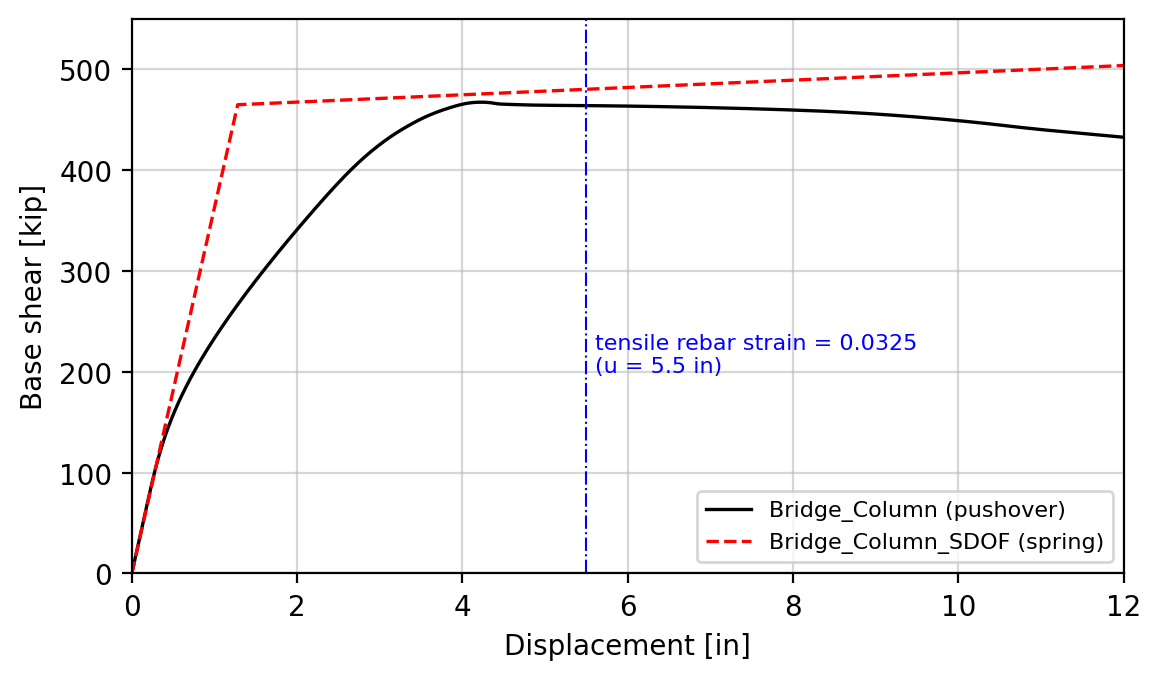
\includegraphics[width=0.55\textwidth]{figures/fig0.png}}\end{figure}

The figure compares the spring with the pushover curve. Two differences are visible:
\begin{itemize}\setlength{\itemsep}{1pt}
\item The spring uses the initial stiffness up to the yield force. The column loses stiffness
      gradually, thus the spring is stiffer than the column between 0.5 in and 4 in.
\item The column loses strength after 5 in because of the P-delta effect. The spring has a positive
      hardening ratio and does not include this effect.
\end{itemize}

The blue line is the displacement at which the maximum tensile strain of the longitudinal rebar
becomes 0.0325 in the pushover. Section 3.3 uses this displacement.

\section{Workflow Objects}

\subsection{Intensity measure}

\codefile{code/code1.txt}

\code{gm\_component\_mode='single\_horizontal'} makes two changes. The GMS stage selects one horizontal
component of each record, and the candidates are the two horizontal components of all records. Each
NLTHA run then gets one file, \code{gm\_1.txt}.

\code{sigma\_component\_func} adds the component-to-component variability $\sigma_C$ of Watson-Lamprey
and Boore (2007) to the standard deviation of the ground motion model:
$\sigma^2_{\ln Sa,\mathrm{Arb}} = \sigma^2_{\ln Sa,\mathrm{GMRotI50}} + \sigma_C^2$.

\subsection{Engineering demand parameter}

The EDP is the maximum absolute displacement of the mass, in inches. \code{MaxDisp} is a concrete
subclass of \code{EDP} in \code{max\_disp.py}. It has the three methods that Section 7.3 of the manual
lists:

\begin{center}
\begin{tabular}{ll}
\toprule
Method & Function in \code{MaxDisp} \\
\midrule
\code{generate\_recorder} & Writes one node displacement recorder for each NLTHA run \\
\code{write\_evaluate\_edp\_and\_helpers} & Writes \code{evaluate\_edp\_1.py}, which returns \code{np.max(np.abs(x))} \\
\code{get\_edp\_strings} & Returns \code{['node\_2']} \\
\bottomrule
\end{tabular}
\end{center}

\codefile{code/code2.txt}

The \code{haz\_req} dictionary of the EDP is the same as in \code{Bridge\_Column}: a lognormal
distribution of EDP given IM, a piecewise linear model for the shape parameter, and a power law for the
scale parameter.

\subsection{Damage state}

\codefile{code/code3.txt}

The damage state is an example. It represents the start of longitudinal bar buckling, which is DS 2 of
\code{Bridge\_Column}.
\begin{itemize}\setlength{\itemsep}{1pt}
\item \textbf{Predictive capacity:} 5.5 in. The predictive capacity of DS 2 in \code{Bridge\_Column} is
      a tensile rebar strain of 0.0325 for the as-designed column. In the pushover, the strain
      becomes 0.0325 at a displacement of 5.5 in.
\item \textbf{Normalized fragility:} \code{lognorm(0.082, 0, 1.03)}. The normalized fragility of DS 2
      in \code{Bridge\_Column} is \code{lognorm(0.201, 0, 1.05)}, and it applies to strain. The
      strain-displacement relation of the pushover changes this strain capacity distribution into a
      displacement capacity distribution. A lognormal fit to that distribution, divided by 5.5 in,
      gives a median of 1.03 and a dispersion of 0.082.
\end{itemize}

The dispersion decreases from 0.201 to 0.082 because the rebar strain increases quickly with the
displacement after the column yields. Between 5 in and 6 in, the strain increases from 0.024 to 0.039.

The predictive capacity is a constant, thus the model does not write a predictor file.

\subsection{Analysis objects}

\codefile{code/code4.txt}

\section{Analysis Driver}

The driver has the same stages as \code{Bridge\_Column}. The three new stages are:

\codefile{code/code5.txt}

The NLTHA stage has 60 runs (6 hazard levels, 10 records for each level). All 60 runs converge.

\section{Results}

All results are for \code{for\_which=['100', '1', '1', '1']}.

\subsection{Seismic hazard}

\codefile{code/code6.txt}

\figpair{figures/fig1.png}{figures/fig2.png}

$Sa(T_1)$ at a mean return period (MRP) of 475 years is 0.364 g. \code{Bridge\_Column} gives 0.341 g
with the geometric mean of the two horizontal components. The increase of 7\% is the effect of
$\sigma_C$.

\subsection{Ground motion selection}

\codefile{code/code7.txt}

\figone{0.6}{figures/fig3.png}

The gray lines are the scaled spectra of the 10 selected components for hazard level 3 (MRP = 475
years). Each spectrum is equal to the target, 0.364 g, at $T_1$. The table shows the selected
components. Each record number (RSN) occurs one time.

\begin{center}
\begin{tabular}{rcll}
\toprule
RSN & Component & File & Scale factor \\
\midrule
1534 & 1 & \code{CHICHI/TCU107-E.AT2} & 1.010 \\
797 & 2 & \code{LOMAP/RIN090.AT2} & 3.731 \\
1288 & 2 & \code{CHICHI/HWA039-N.AT2} & 1.426 \\
1703 & 1 & \code{NORTH392/00BN22E.AT2} & 1.779 \\
1389 & 2 & \code{CHICHI/KAU074-N.AT2} & 3.137 \\
164 & 2 & \code{IMPVALL/H-CPE237.AT2} & 1.432 \\
360 & 2 & \code{COALINGA/H-VC1090.AT2} & 1.267 \\
1359 & 2 & \code{CHICHI/KAU015-N.AT2} & 3.998 \\
1348 & 1 & \code{CHICHI/ILA064-N.AT2} & 2.935 \\
1308 & 2 & \code{CHICHI/ILA002-W.AT2} & 1.542 \\
\bottomrule
\end{tabular}
\end{center}

\subsection{Nonlinear time-history analysis}

The table shows the maximum displacement of the 10 runs at each hazard level. The yield displacement
of the spring is 1.28 in.

\begin{center}
\begin{tabular}{crrrrr}
\toprule
Hazard level & MRP [years] & $Sa(T_1)$ [g] & Minimum [in] & Median [in] & Maximum [in] \\
\midrule
1 & 72 & 0.176 & 1.49 & 1.71 & 2.19 \\
2 & 224 & 0.280 & 1.84 & 2.09 & 3.56 \\
3 & 475 & 0.364 & 1.86 & 2.77 & 5.63 \\
4 & 975 & 0.457 & 1.97 & 3.34 & 6.07 \\
5 & 2475 & 0.598 & 2.72 & 3.77 & 13.0 \\
6 & 4975 & 0.719 & 3.00 & 4.98 & 70.3 \\
\bottomrule
\end{tabular}
\end{center}

One run at hazard level 6 gives 70.3 in. The spring has a hardening ratio of 0.01 and no P-delta
effect, thus the displacement can increase in one direction without a limit. This run increases the
dispersion at hazard level 6.

\textbf{Spring hysteresis.} The script \code{extract\_single\_nltha.py} extracts one NLTHA run into a
new folder, with two more recorders for the spring. The name of the folder is
\code{Bridge\_Column\_SDOF\_extract\_OpenSeesPy}. It then
runs the analysis and plots the spring force against the spring deformation.

\codefile{code/code11.txt}

\figone{0.95}{figures/fig9.png}

The figure shows six runs, made with different values of \code{for\_which}. The top row is the run with
the median EDP at hazard levels 1, 3 and 6. The bottom row is the run with the largest EDP at hazard
levels 1 and 3, and the run with the second largest EDP at hazard level 6. The figure does not show
the 70.3 in run of hazard level 6, thus all panels can have the same axis limits. The maximum deformation of each extracted run is equal to the EDP value of the workflow.

The loops show the bilinear \code{Steel01} behavior: the yield force is 465 kip, and the unloading
stiffness is equal to the initial stiffness. The six panels have the same axis limits.

\subsection{Demand hazard}

\codefile{code/code8.txt}

\figpair{figures/fig4.png}{figures/fig5.png}

The left figure shows the lognormal distributions of the EDP at the six hazard levels. The right
figure shows the three lognormal parameters as a function of the IM. The shape parameter at hazard
level 6 is 0.84 because of the 70.3 in run.

\codefile{code/code9.txt}

\begin{minipage}[c]{0.56\textwidth}
\fbox{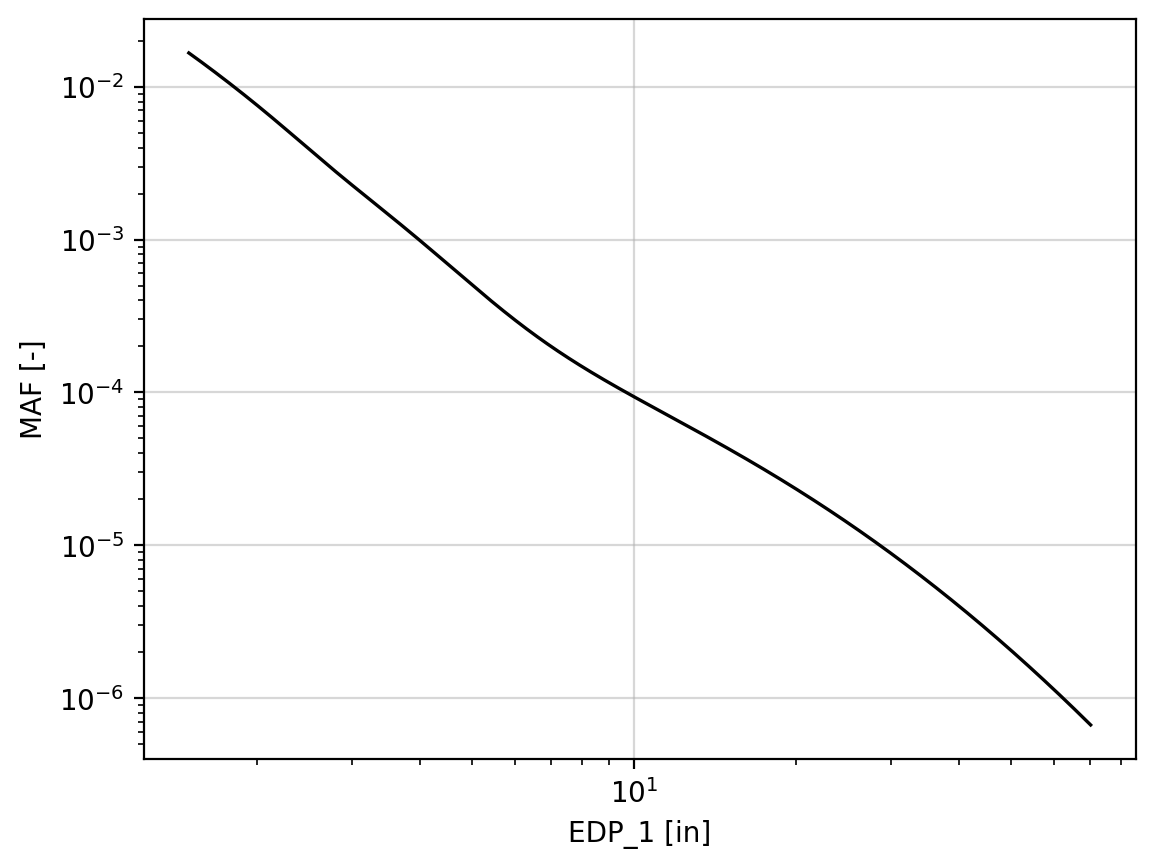
\includegraphics[width=0.95\textwidth]{figures/fig6.png}}
\end{minipage}\hfill
\begin{minipage}[c]{0.4\textwidth}
\centering
\begin{tabular}{rr}
\toprule
Displacement [in] & MRP of exceedance [years] \\
\midrule
2.0 & 133 \\
3.0 & 441 \\
4.0 & 1010 \\
5.5 & 2616 \\
8.0 & 6773 \\
\bottomrule
\end{tabular}
\end{minipage}

\subsection{Damage hazard}

\codefile{code/code10.txt}

\figpair{figures/fig7.png}{figures/fig8.png}

The left figure is the fragility function in displacement units. Its median is
$1.03 \times 5.5 = 5.67$ in. The right figure shows the seismic hazard curve (blue) and the
contribution of each IM value to the damage hazard (red).

\textbf{The MRP of the damage state is 2762 years.} The largest contributions come from the IM range
of the six hazard levels (light blue area). Thus the NLTHA results, and not the extrapolation of the
demand model, control the result.

\subsection{Comparison with Bridge\_Column}

\begin{center}
\begin{tabular}{lrr}
\toprule
 & \code{Bridge\_Column} (DS 2) & \code{Bridge\_Column\_SDOF} \\
\midrule
$T_1$ [s] & 0.9403 & 0.9405 \\
$Sa(T_1)$ at MRP = 475 years [g] & 0.341 & 0.364 \\
MRP of the damage state [years] & 449 & 2762 \\
\bottomrule
\end{tabular}
\end{center}

The period and the hazard agree. The MRP of the damage state is 6.2 times larger for the SDOF. The two
examples have these differences, and each one can change the MRP:
\begin{itemize}\setlength{\itemsep}{1pt}
\item \code{Bridge\_Column} gets two horizontal components and the vertical component. The SDOF gets one
      horizontal component.
\item The displacement capacity and its fragility come from a monotonic pushover in one direction.
      In a time-history analysis with cyclic loads in two directions, the rebar strain can become
      0.0325 at a smaller displacement.
\item The spring is stiffer than the column between 0.5 in and 4 in, and it has no P-delta effect.
\end{itemize}

This document does not quantify the effect of each difference. Thus the SDOF damage state is an
example of the workflow. It is not a calibrated replacement for DS 2 of \code{Bridge\_Column}.

\section{How to Run the Example}

Run \code{analysis\_driver.py} from the folder \code{scripts/examples/Bridge\_Column\_SDOF}, with the
repository root on \code{PYTHONPATH}. PyPBEE writes the results to
\code{PyPBEE\_Work\_Dir/Bridge\_Column\_SDOF\_Work\_Dir}.

Two messages on the console are expected:
\begin{itemize}\setlength{\itemsep}{1pt}
\item OpenSees prints a warning about the \code{-fullGenLapack} eigen solver. The default solver
      does not work for a model with one degree of freedom.
\item PyPBEE prints ``Damping information not found''. The damping is in \code{ops\_model.py},
      because the modal damping of PyPBEE uses the default eigen solver.
\end{itemize}

\section{References}

Watson-Lamprey, J. A., and Boore, D. M. (2007). Beyond $Sa_{GMRotI}$: Conversion to $Sa_{Arb}$,
$Sa_{SN}$, and $Sa_{MaxRot}$. \textit{Bulletin of the Seismological Society of America}, 97(5),
1511-1524.

\end{document}
